\documentclass[../lab2.tex]{subfiles}

\begin{document}
    In questo caso si analizza uno scenario in cui dal Pc Live Linux si esegue il comando \textit{ping} 
    ad un dispositivo connesso via WiFi (nel nostro caso una firestick TV amazon, 
    frequenza di connessione 2.4 GHz, Wi-Fi 5 (IEEE 802.11ac))

    \begin{center}
        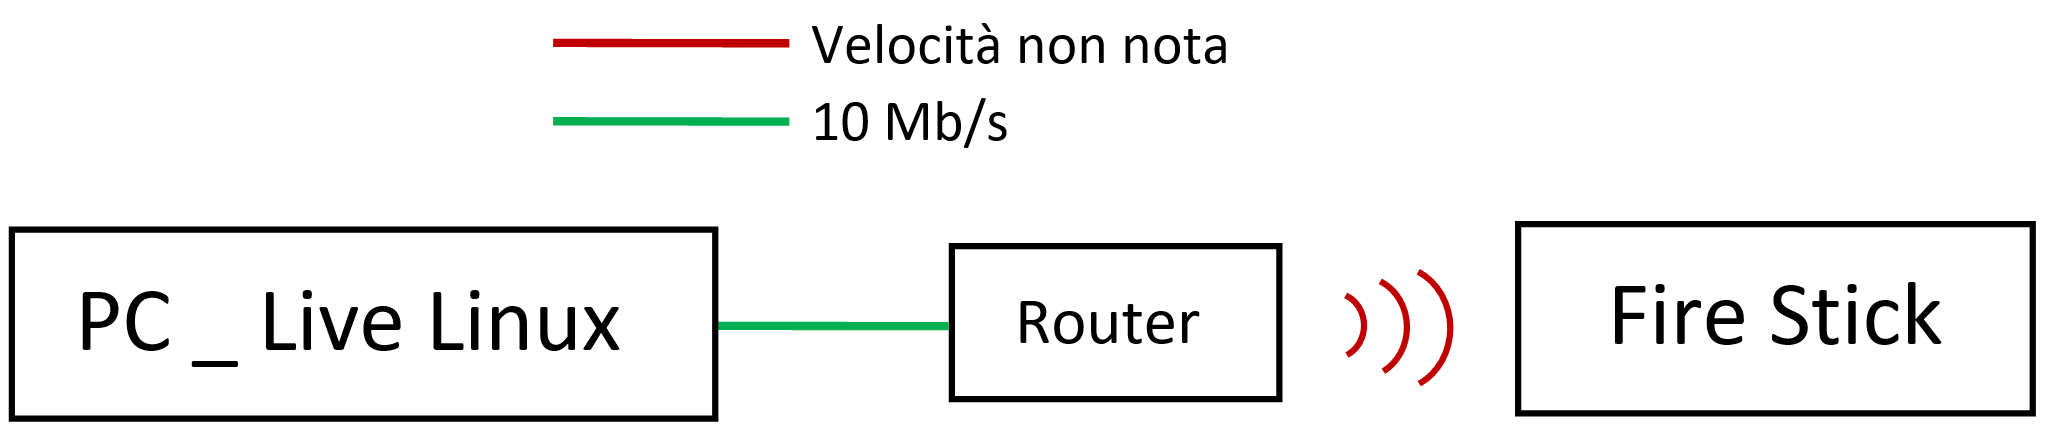
\includegraphics[width=0.5\linewidth]{conf3.png}
    \end{center}
\end{document}